% Statistical Foundations of Prior-Data Fitted Networks --- fm4sd seminar talk
% Beamer / metropolis. Build with: make  (latexmk + lualatex)
\documentclass[aspectratio=169,10pt]{beamer}

\usetheme{metropolis}
\metroset{progressbar=frametitle, numbering=fraction, block=fill}

\usepackage[T1]{fontenc}
\usepackage{booktabs}
\usepackage{amsmath,amssymb}
\usepackage{tikz}
\usetikzlibrary{positioning,arrows.meta,fit,backgrounds,calc,matrix}
\usepackage{pgfplots}
\pgfplotsset{compat=1.18}
\usepackage{xcolor}
\usepackage{xurl}

% --- palette ---------------------------------------------------------------
\definecolor{accent}{HTML}{C1121F}
\definecolor{ink}{HTML}{2B2D42}
\definecolor{muted}{HTML}{6C757D}
\definecolor{good}{HTML}{2A9D8F}
\setbeamercolor{frametitle}{bg=ink}
\setbeamercolor{background canvas}{bg=white}
\setbeamercolor{normal text}{fg=ink, bg=white}
\setbeamercolor{progress bar}{fg=accent}
\setbeamercolor{alerted text}{fg=accent}

\newcommand{\hl}[1]{{\color{accent}\textbf{#1}}}
\newcommand{\gd}[1]{{\color{good}\textbf{#1}}}
\newcommand{\mut}[1]{{\color{muted}#1}}

% compact citation marks (we keep refs informal on slides)
\newcommand{\cit}[1]{{\scriptsize\color{muted}[#1]}}

\title{Statistical Foundations of Prior-Data Fitted Networks \cit{Nagler '23}}
\author{Salih \underline{Bora} Öztürk \;\&\; \underline{Gurmeher} Singh Puri}
\institute{University of Freiburg \\ \footnotesize Seminar on Foundation Models for Structured Data - SS26 \\ Group 4}
\date{19 June 2026}
\titlegraphic{%
  \begin{tikzpicture}[remember picture, overlay]
    \node[anchor=south east] at ([xshift=-8mm,yshift=6mm]current page.south east) {
\includegraphics[height=3cm]{img/logo-ufr.png}};
  \end{tikzpicture}%
}

\begin{document}

\maketitle

% --- What does PFN stand for? --------------------------------------------
% arrow lives inside the (otherwise blank) dark title strip, pointing right -> left
% width 9cm, centered -> spans the P..N letters (which sit at x = +/-4.5, also centered)
\begin{frame}{\makebox[\linewidth][c]{\raisebox{1.2mm}[0pt][0pt]{\tikz[baseline]{%
    \draw[-{Stealth[length=5mm,width=6mm]}, line width=2.4pt, white] (10.6,0) -- (0,0);}}}}
\vfill
\centering
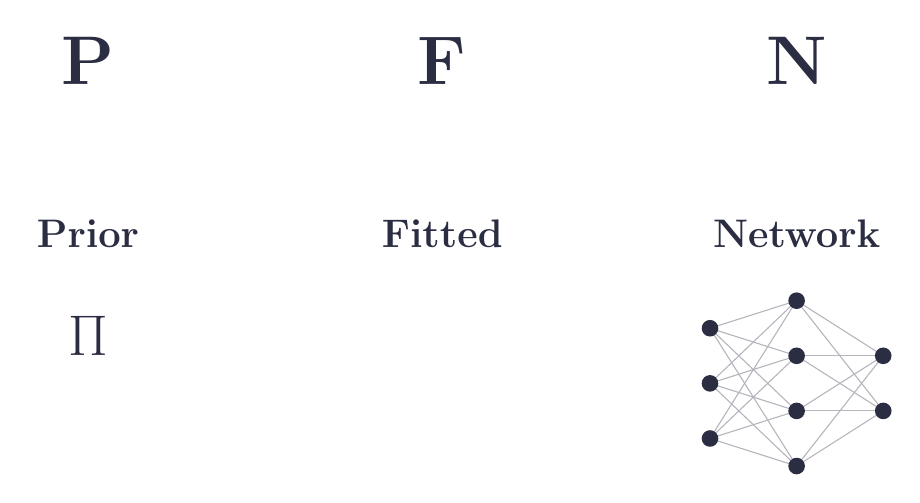
\begin{tikzpicture}[>=Stealth]
  % huge letters P F N
  \node[font=\fontsize{88}{88}\selectfont\bfseries, ink] (P) at (-4.5,0) {P};
  \node[font=\fontsize{88}{88}\selectfont\bfseries, ink] (F) at ( 0  ,0) {F};
  \node[font=\fontsize{88}{88}\selectfont\bfseries, ink] (N) at ( 4.5,0) {N};

  % --- Network (under N, shown from the start) ---------------------------
  \node[font=\Large\bfseries, ink] (Nw) at (4.5,-2.2) {Network};
  % small, label-free neural net under "Network"
  \begin{scope}[shift={(4.5,-4.1)}]
    \foreach \i in {0,1,2}   \coordinate (i\i) at (-1.1,{(\i-1)*0.7});
    \foreach \i in {0,1,2,3} \coordinate (h\i) at ( 0  ,{(\i-1.5)*0.7});
    \foreach \i in {0,1}     \coordinate (o\i) at ( 1.1,{(\i-0.5)*0.7});
    \foreach \i in {0,1,2}   \foreach \j in {0,1,2,3} \draw[ink!35,line width=0.4pt] (i\i)--(h\j);
    \foreach \i in {0,1,2,3} \foreach \j in {0,1}     \draw[ink!35,line width=0.4pt] (h\i)--(o\j);
    \foreach \i in {0,1,2}   \fill[ink] (i\i) circle(3pt);
    \foreach \i in {0,1,2,3} \fill[ink] (h\i) circle(3pt);
    \foreach \i in {0,1}     \fill[ink] (o\i) circle(3pt);
  \end{scope}

  % --- Fitted (under F, click 1) -----------------------------------------
  \onslide<2->{\node[font=\Large\bfseries, ink] at (0,-2.2) {Fitted};}

  % --- Prior + its symbol (under P, click 2) -----------------------------
  \onslide<3->{%
    \node[font=\Large\bfseries, ink] (Pr) at (-4.5,-2.2) {Prior};
    \node[font=\huge, ink] at (-4.5,-3.5) {$\Pi$};
  }
\end{tikzpicture}
\vfill
\end{frame}

% --- next slide (empty) ---------------------------------------------------
\begin{frame}
\end{frame}

\begin{frame}{PFNs approximate PPD}
\end{frame}

% --- next slide (empty) ---------------------------------------------------
\begin{frame}
\end{frame}

\begin{frame}{Bayesian view}
\end{frame}

\begin{frame}{PFNs training}
\end{frame}

\begin{frame}{PFNs approximate PPD}
\end{frame}

\end{document}
